\documentclass[11pt]{article}
\usepackage{ece786}

%%%%%%%%%%%%%%%%%%%% name/id
\rfoot{\small Brian Park | 200190057}


%%%%%%%%%%%%%%%%%%%% Course/HW info
\newcommand*{\instr}{Huiyang Zhou}
\newcommand*{\term}{Spring 2023}
\newcommand*{\coursenum}{ECE 786}
\newcommand*{\coursename}{Advanced Computer Architecture: Data Parallel Processors}
\newcommand*{\hwnum}{1}

\rhead{\LARGE   \fontfamily{lmdh}\selectfont	HW \hwnum}

\lfoot{\small \coursenum, \term, HW \hwnum}

%%%%%%%%%%%%%%%%%%%%%%%%%%%%%% Document Start %%%%%%%%%%%%%%%%%
\begin{document}
%All the questions are from Computer Architecture: A Quantitative Approach, 6th Ed., the textbook of ECE563.

%%%%%%%%%%%%%%%%%%%%%%%%%%%%%%%%%%%%%%%%%%%%%%%%%%%%%%%%%%%%%%%%%%%%%%%%%%%%%%%%%%%%%%%%
% Question 1
%%%%%%%%%%%%%%%%%%%%%%%%%%%%%%%%%%%%%%%%%%%%%%%%%%%%%%%%%%%%%%%%%%%%%%%%%%%%%%%%%%%%%%%%
\section*{1. C.8}
 %1. C.8 (There is a typo in the question: Figure C.21 should be Figure C.22).
 [15] $<$C.5$>$ Construct a table like that shown in Figure C.22 to check for WAW stalls in the RISC V FP pipeline of Figure C.30. Do not consider FP divides.

\begin{figure}[H]
	\centerline{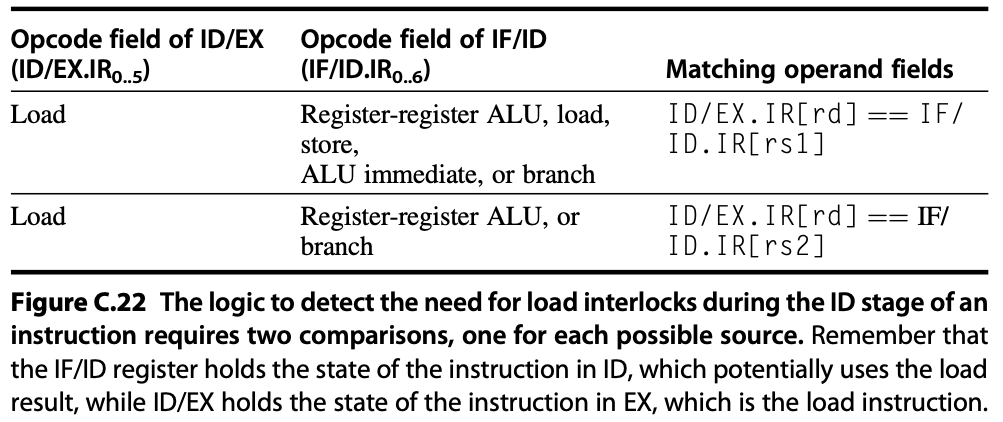
\includegraphics[width=5in]{figures/figurec22.png}}
\end{figure}

\begin{figure}[H]
	\centerline{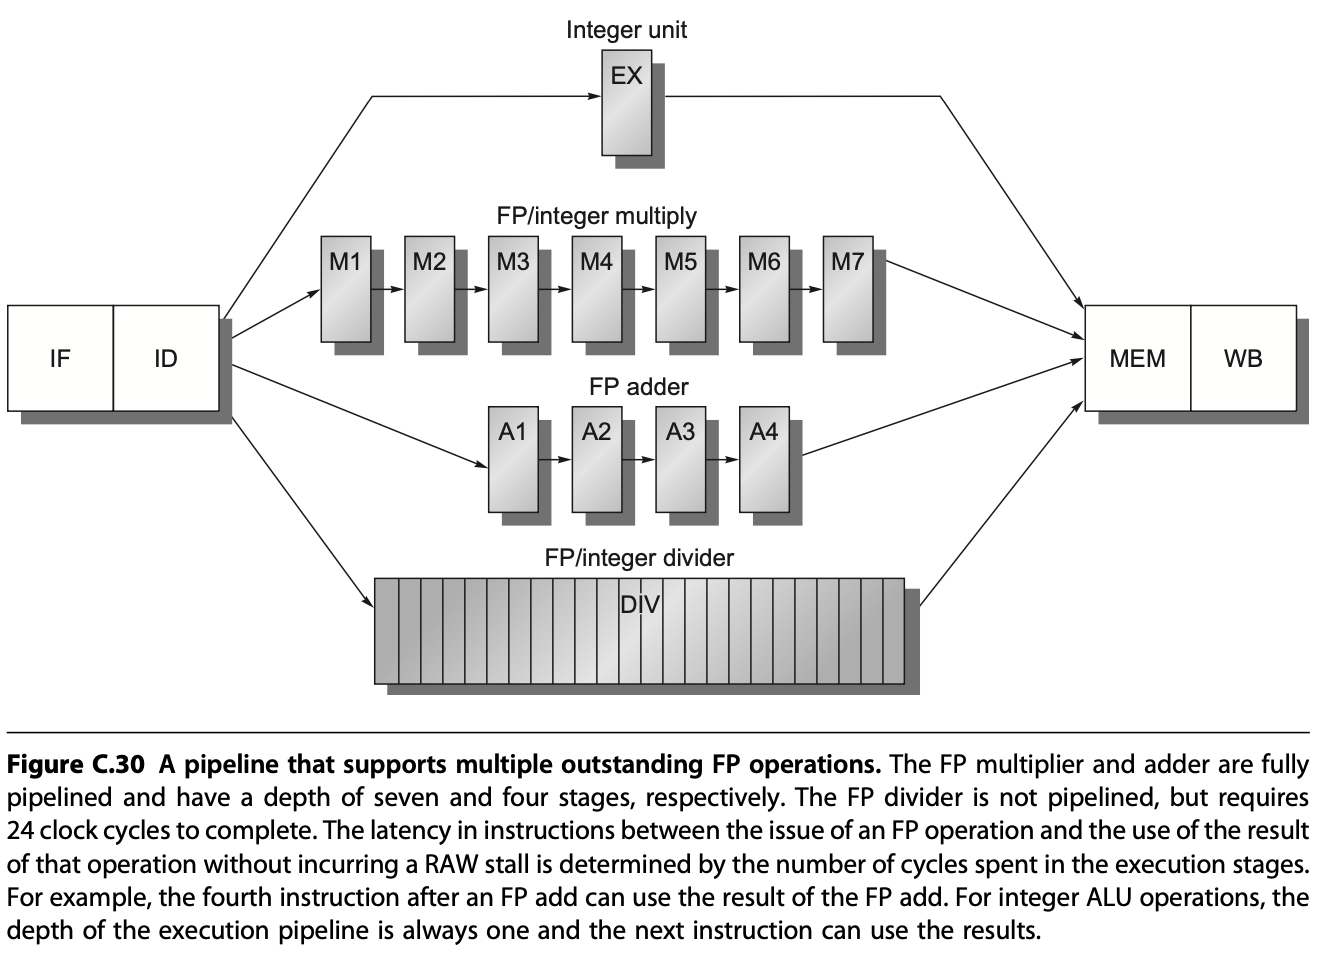
\includegraphics[width=5in]{figures/figurec30.png}}
\end{figure}
\newpage

\begin{Answer}
	Answer is in Table 1 above. Essentially, any case where there is a instruction with lower latency in IF/ID than the one in ID/EX will hit a WAW dependency, because the newer instruction in IF/ID can finish earlier than the older one in ID/EX. Thus a stall is needed. The table lists those scenarios. Since enumerating all of the stages is tedious, it's also important to mention that ID/EX also includes the
	\textit{pipelined registers within the execution unit}.
\end{Answer}

\begin{table}
	\caption{Detecting WAW Stalls at the ID Stage} % title of Table
	\centering % used for centering table
	\begin{tabular}{c c c} % centered columns (4 columns)
		\hline\hline %inserts double horizontal lines
		Opcode field of ID/EX & Opcode field of IF/ID      & Matching operand fields             \\ [0.5ex] % inserts table
		%heading
		\hline % inserts single horizontal line
		FMUL                  & FADD                       & \verb|ID/EX.IR[rd] == IF/ID.IR[rd]| \\
		(Integer) MUL         & Integer ALU/ ALU immediate & \verb|ID/EX.IR[rd] == IF/ID.IR[rd]| \\
		FADD                  & Load                       & \verb|ID/EX.IR[rd] == IF/ID.IR[rd]| \\
		FMUL                  & Load                       & \verb|ID/EX.IR[rd] == IF/ID.IR[rd]| \\
		[1ex] % [1ex] adds vertical space
		\hline %inserts single line
	\end{tabular}
	\label{table:nonlin} % is used to refer this table in the text
\end{table}

%If integer, nothing really has to be done.

%NOTES:

%WAW hazard is also know as Output-dependence,
%where an example is as follows: \\

%\begin{verbatim}
%%add r3, r1, r2
%%add r3, r6, r7
%\end{verbatim}



\newpage
%%%%%%%%%%%%%%%%%%%%%%%%%%%%%%%%%%%%%%%%%%%%%%%%%%%%%%%%%%%%%%%%%%%%%%%%%%%%%%%%%%%%%%%%
% Question 2
%%%%%%%%%%%%%%%%%%%%%%%%%%%%%%%%%%%%%%%%%%%%%%%%%%%%%%%%%%%%%%%%%%%%%%%%%%%%%%%%%%%%%%%%
\section*{2. C.9.a}
 %2. C.9.a

 [20/22/22] $<$C.4, C.6$>$ In this exercise, we will look at how a common vector loop runs on statically and dynamically scheduled versions of the RISC V pipeline. The loop is the so-called DAXPY loop (discussed extensively in Appendix G) and the central operation in Gaussian elimination. The loop implements the vector operation $Y=a*X+Y$ for a vector of length 100. Here is the MIPS code for the loop:

\begin{verbatim}
foo:    fld    f2, 0(x1)    ; load X(i)
        fmul.d f4, f2, f0   ; multiply a*X(i)
        fld    f6, 0(x2)    ; load Y(i)
        fadd.d f6, f4, f6   ; add a*X(i) + Y(i)
        fsd    0(x2), f6    ; store Y(i)
        addi   x1, x1, 8    ; increment X index
        addi   x2, x2, 8    ; increment Y index
        sltiu  x3, x1, done ; test if done
        bnez   x3, foo      ; loop if not done
\end{verbatim}

For parts (a) to (c), assume that integer operations issue and complete in 1 clock cycle (including loads) and that their results are fully bypassed. You will use the FP latencies (only) shown in Figure C.29, but assume that the FP unit is fully pipelined. For scoreboards below, assume that an instruction waiting for a result from another function unit can pass through read operands at the same time the result is written. Also assume that an instruction in WB completing will allow a currently active instruction that is waiting on the same functional unit to issue in the same clock cycle in which the first instruction completes WB.

a. [20]$<$C.5$>$ For this problem, use the RISCV pipeline of Section C.5 with the pipeline latencies from Figure C.29, but a fully pipelined FP unit, so the initiation interval is 1. Draw a timing diagram, similar to Figure C.32, showing the timing of each instruction's execution. How many clock cycles does each loop iteration take, counting from when the first instruction enters the WB stage to when the last instruction enters the WB stage?
\newpage

\begin{Answer}

	For this solution, I assumed in-order memory WB. It takes (24 - 4) 20 clock cycles to do one iteration of loop. Stalls also happened before execution in this solution, and since pipeline is fully bypassed, instructions greedily executed once results were available in the pipeline registers. For ALU/EX units, EX/MEM registers are fully bypassed to the next stage. Since \verb|ld| has data ready at the end of the cycle in the MEM stage, we bypass MEM/WB registers to the EX stage when needed, instead of EX/MEM. The timing diagram is shown below.
	\begin{verbatim}
Instruction           | 1  | 2  | 3  | 4   | 5     | 6     | 7     | 8     | 9     |
1. fld f2, 0(x1)      | IF | ID | EX | MEM | WB    |       |       |       |       |
2. fmul.d f4, f2, f0  |    | IF |    | ID  | FMUL1 | FMUL2 | FMUL3 | FMUL4 | FMUL5 |
3. fld f6, 0(x2)      |    |    |    | IF  | ID    |       |       |       |       |
4. fadd.d f6, f4, f6  |    |    |    |     | IF    |       |       |       |       |
5. fsd 0(x2), f6      |    |    |    |     |       |       |       |       |       |
6. addi x1, x1, 8     |    |    |    |     |       |       |       |       |       |
7. addi x2, x2, 8     |    |    |    |     |       |       |       |       |       |
8. sltiu x3, x1, done |    |    |    |     |       |       |       |       |       |
9. bnez x3, foo       |    |    |    |     |       |       |       |       |       |


Instruction           | 10    | 11    | 12  | 13    | 14    | 15    | 16    | 17    |
1. fld f2, 0(x1)      |       |       |     |       |       |       |       |       |
2. fmul.d f4, f2, f0  | FMUL6 | FMUL7 | MEM | WB    |       |       |       |       |
3. fld f6, 0(x2)      |       |       | EX  | MEM   | WB    |       |       |       |
4. fadd.d f6, f4, f6  |       |       | ID  |       | FADD1 | FADD2 | FADD3 | FADD4 |
5. fsd 0(x2), f6      |       |       | IF  |       | ID    |       |       |       |
6. addi x1, x1, 8     |       |       |     |       | IF    |       |       |       |
7. addi x2, x2, 8     |       |       |     |       |       |       |       |       |
8. sltiu x3, x1, done |       |       |     |       |       |       |       |       |
9. bnez x3, foo       |       |       |     |       |       |       |       |       |

Instruction           | 18  | 19  | 20  | 21  | 22  | 23  | 24 |
1. fld f2, 0(x1)      |     |     |     |     |     |     |    |
2. fmul.d f4, f2, f0  |     |     |     |     |     |     |    |
3. fld f6, 0(x2)      |     |     |     |     |     |     |    |
4. fadd.d f6, f4, f6  | MEM | WB  |     |     |     |     |    |
5. fsd 0(x2), f6      | EX  | MEM | WB  |     |     |     |    |
6. addi x1, x1, 8     | ID  | EX  | MEM | WB  |     |     |    |
7. addi x2, x2, 8     | IF  | ID  | EX  | MEM | WB  |     |    |
8. sltiu x3, x1, done |     | IF  | ID  | EX  | MEM | WB  |    |
9. bnez x3, foo       |     |     | IF  | ID  | EX  | MEM | WB |
\end{verbatim}

\end{Answer}
\newpage

\end{document}